\documentclass{article}
\usepackage{ctex}
\usepackage{xltxtra}
\usepackage{graphicx}
\usepackage{xcolor}
\usepackage{listings}
\usepackage{amsmath}
\usepackage{subfigure}
\usepackage{geometry}
\usepackage{amssymb}
\geometry{a4paper,left=2cm,right=2cm,top=2cm,bottom=2cm}
\graphicspath{{../fig/}}

\lstset{language=C++}
\lstset{
    numbers=left, 
    numberstyle= \tiny,
    basicstyle = \small, 
    keywordstyle= \color{ blue!70},
    commentstyle= \color{red!50!green!50!blue!50}, 
    frame=shadowbox, 
    rulesepcolor= \color{ red!20!green!20!blue!20} ,
    escapeinside=``,
    xleftmargin=2em, aboveskip=1em,
    breaklines = true,
    columns  = fixed,
    framexleftmargin=2em
}

\title{{\bf Project: Splines Interpolation}}
\author{陈震翔\\3210103924 信息与计算科学}

\date{}

\begin{document}

\maketitle

\section{Introduction}
In this project, I impletement arbitrary dimension piecewise-polynomial splines(liner and cubic) and B-splines(arbitrary order), but quadratic and cubic cardinal B-splines is only for 1 dimension, and a abstract function class, you can use them just like below:
\begin{lstlisting}
//defined in splines.h enum BCType{ myDefault2, complete, nature, second, notAKnot, periodic };pp-Form support all but B-Form don't support notKnot and periodic
constexpr int Dim;
constexpr int Order;
class youFunction: Function<Dim>{
    //override pure virtual function val() to defined your Function 
    //you also can choose to override the function diffval() to define a more precise derivative instead of the numerical derivative which have impletemented
};
vector<double> knots;
double left, right;//interval for cardinal B-splines
BCType bctype;
youFunction f;
vector<Vector<double,Dim> > points;// if Dim == 1, we need use vector<double>
vector<Vector<double,Dim> > boundaryCondition;// same as above
ppSpline<Order,Dim> ppS;
BSpline<Order,Dim> BS;
CardinalBSpline<Order> CBS;
//ppS and BS have the same process for fit a curve;
ppS.setKnots(knots);//or you can set knots while you define the ppS with initialized list{knots}
CBS.setInterval(left,right);
ppS.fitCurve(f,bctype);//fit function
ppS.fitCurve(points,bctype,boundaryCondition);//fit points in Dim dimension space
//As for dimension higher than 1, fitCurve() will return a double type for the right of cumulative chordal length
CBS.fitCurve(f);//only support fit function
double x;
cout << ppS(x) << endl;//get the value of splines at x; 
\end{lstlisting}

More details you can get in the design document(design.pdf).

\newpage

\section{Problem A}
\subsection{Plot Results}
In this assignment, I test all the boundary condition of cubic-spline interpolation(use piecewise polynomial form) of the function
$$f(x)=\frac{1}{1+25x^2}$$

The result is below:
\begin{figure}[h]
    \centering
    \subfigure[complete]{
        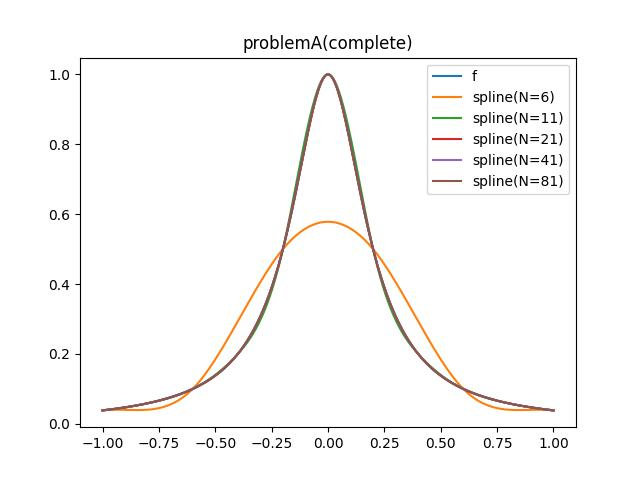
\includegraphics[scale=0.45]{problemA(complete).jpg}
    }
    \quad
    \subfigure[nature]{
    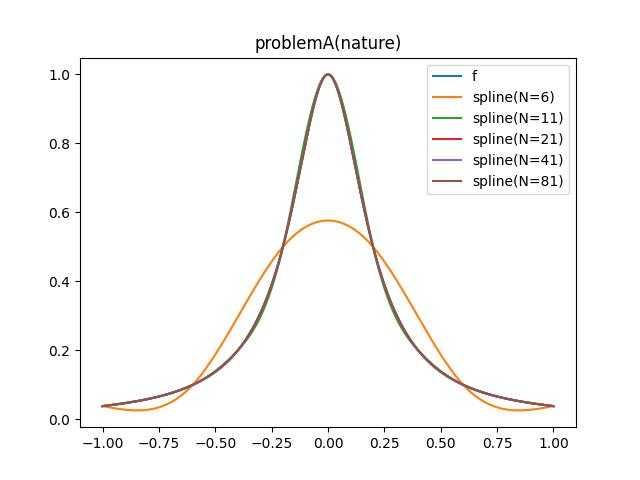
\includegraphics[scale=0.45]{problemA(nature).jpg} 
    }
    \quad
    \subfigure[second]{
    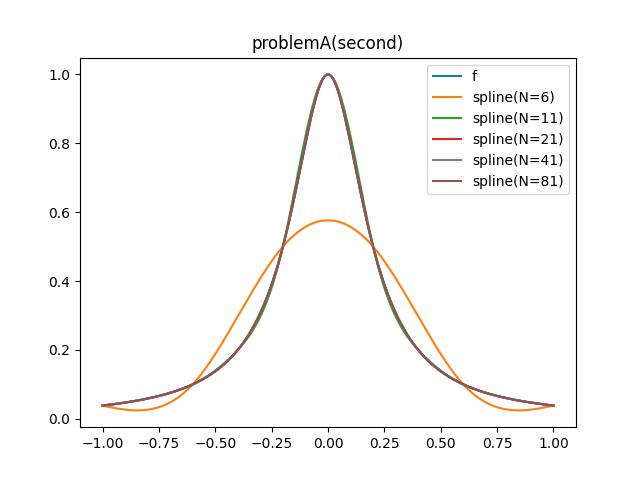
\includegraphics[scale=0.45]{problemA(second).jpg}
    }
    \quad
    \subfigure[notAKnot]{
    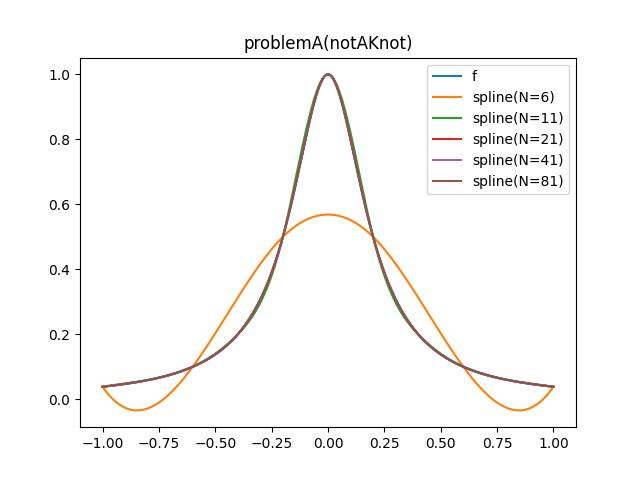
\includegraphics[scale=0.45]{problemA(notAKnot).jpg}
    }
    \subfigure[periodic]{
    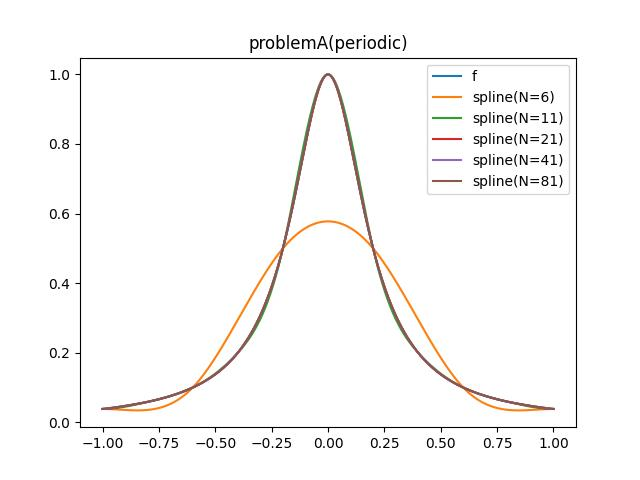
\includegraphics[scale=0.45]{problemA(periodic).jpg}
    }
\caption{Results of cubic-spline interpolation for $f(x)=\frac{1}{1+25x^2}$}
\end{figure}

We can see that while number of knots is larger than 11, all condition can fit the function well, which is free of the wide oscillations in the Runge phenomenon. And as for N = 6, the condition, not-a-knot, flucuate more seriously between first two and last two knots than other condition obviously, this maybe because it give a extra requirement at second and penult knot. 

\subsection{Errors Analysis}
\begin{figure}[h]
    \centering
    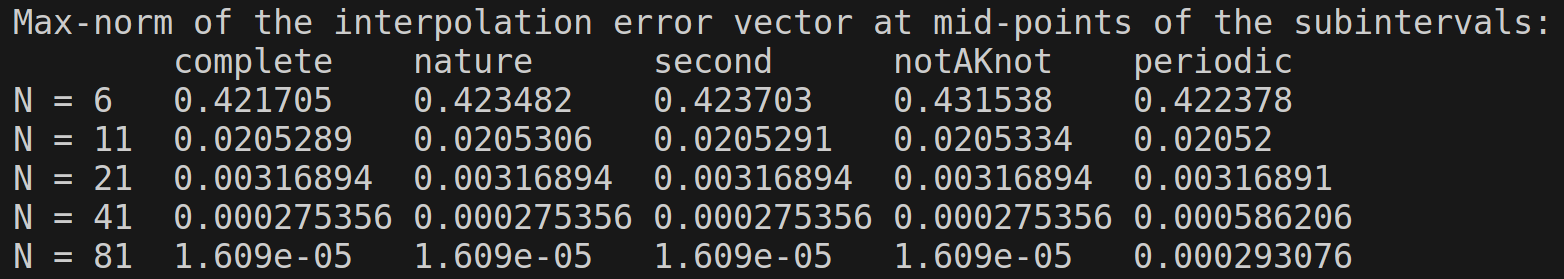
\includegraphics[width=\linewidth]{problemAerrors.png}
    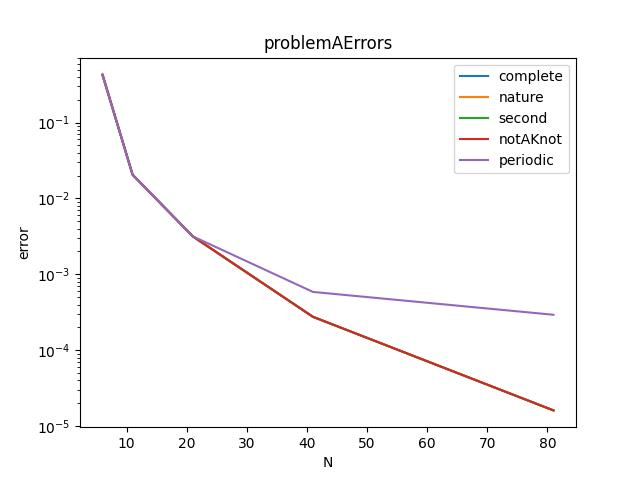
\includegraphics[width=0.7\linewidth]{problemAErrors.jpg}
    \caption{max-norm errors at mid-points of subintervals}
\end{figure}

We can see that the errors of cubic-spline interpolation for all boundary condition all decline rapidly, with $N$ going large.But for condition periodic, the errors decline become slow while N is too large, I think it may be because the function $f(x)=\frac{1}{1+25x^2}$ is actually not a periodic function.

As for convergence rate, at first, we have the therom
$$Suppose\ f \in \mathcal{C}^4:[a,b]\rightarrow \mathbb{R},\ s\in\mathbb{S}_{3}^{2} \ fit\ in\ f\ with\ condition\ complete\ or\ specified\ second\ derivative$$
$$we\ have\ |f(x)-s(x)|\leq\frac{1}{16}h^4max_{x\in[a,b]}|f^{(4)}(x)|,\ where\ h=max_{i=1}^{N-1}|x_{i+1}-x_i|$$
Therefore, the errors should decline in a rate of $O(1/N^4)$, we multiply $N^4$ for each errors, then we get the reult below:
\begin{figure}[h]
    \centering
    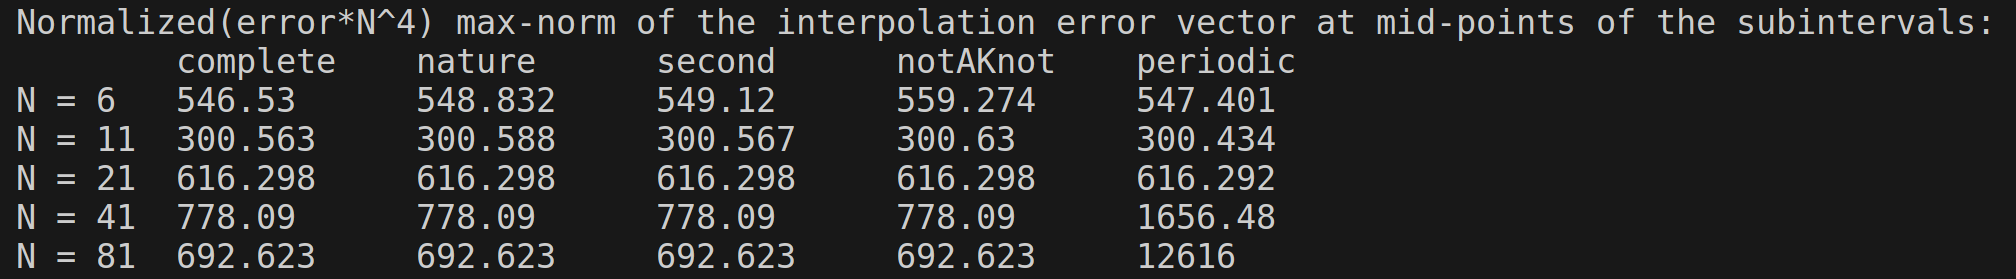
\includegraphics[width=0.8\linewidth]{problemAnorerrors.png}
\end{figure}
\begin{figure}[h]
    \centering
    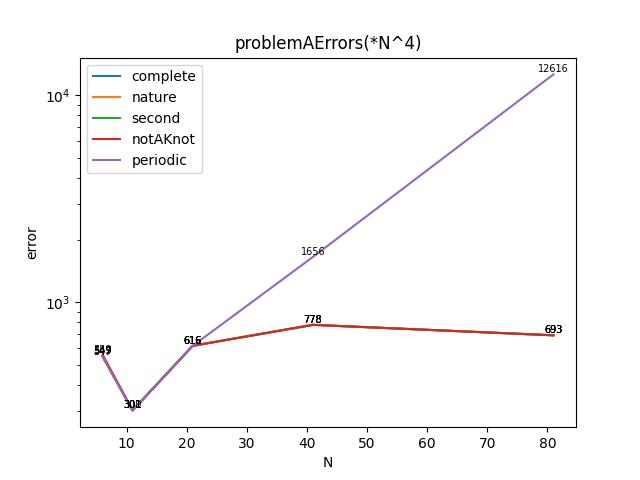
\includegraphics[width=0.7\linewidth]{problemAErrors(*N^4).jpg}
    \caption{normalized max-norm errors}
\end{figure}
\newpage
We can see, except the condition periodic, the others are all in the same order of magnitudes, which verifies the idea above.
\section{Problem BCD}
\begin{figure}[h]
    \centering
    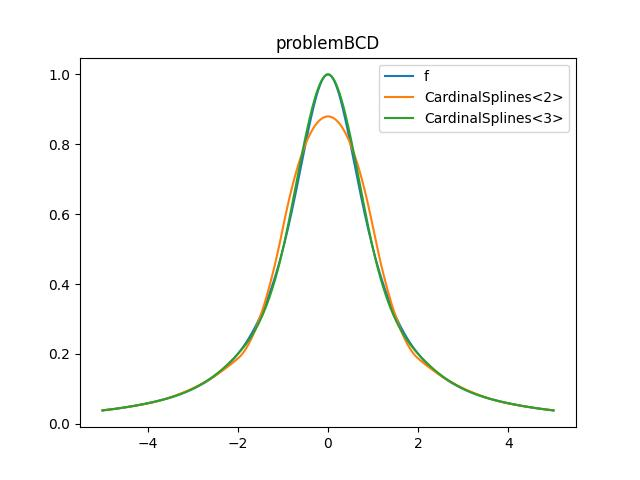
\includegraphics[width = 0.65\linewidth]{problemBCD.jpg}
    \caption{quadratic and cubic cardinal B-splines against $f(x)=\frac{1}{1+x^2}$}
\end{figure}
\newpage

The errors at $x\in\{-3.5,-3,-0.5,0,0.5,3,3.5\}$ of two cardinal B-splines are below:
\begin{figure}[h]
    \centering
    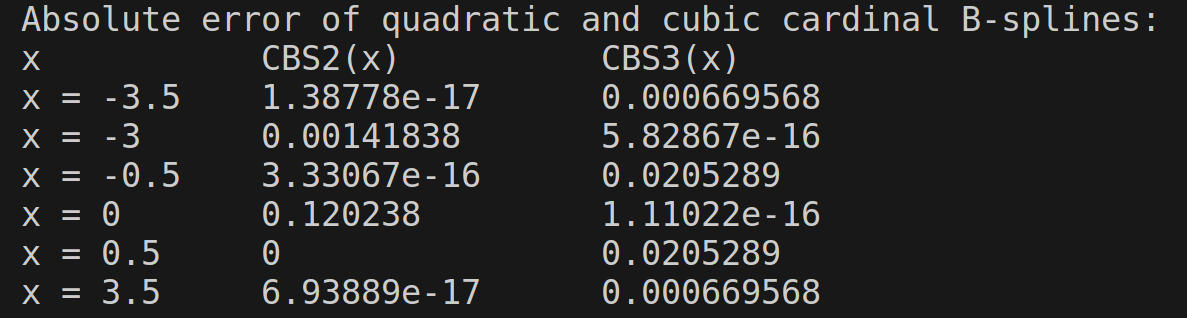
\includegraphics[width=0.5\linewidth]{problemBerrors.png}
\end{figure}

We can find that for quadratic cardinal B-splines at $x=-3.5,-0.5,0.5,3.5$ and for cubic cardinal B-splines at $x=-3,0,3$, the errors colse to machine precision or even be equal to $0$. That's because that quadratic or cubic cardinal B-splines interpolate at these points and its values at these knots are equal to $f(x)$, but the floating-point number system in computer has errors, so the errors is colse to machine precision.

From the figure above and the errors outputted, the cubic cardinal B-splines is more accurate.
\section{Problem E}
At first, transform curve function $$x^2+(\frac{3}{2}y-\sqrt{|x|})^2=3$$
to the form of a parameter function of components
$$
\begin{cases}
x(\theta) = \sqrt{3}sin\theta\\
y(\theta) = \frac{2}{3}(\sqrt{3}cos\theta + \sqrt{|\sqrt{3}sin\theta|})\\
\theta \in [0,2\pi]
\end{cases}
$$

We can find that at points $(0, \pm\frac{2\sqrt{3}}{3})$, any order derivative of component $y(\theta)$ isn't existed, and it will tend to $\pm\infty(\mp\infty)$ approaching from right(left). So these two points is the characteristic points, which must be included in knots, of this curve. And it is obviously that we need to try our best to describe the property of curve near these two points.

Firstly, how describe the derivative of curve is not existed at these two points. For this property, we can't choose complete or specified second derivative as boundary condition(because it need the information of derivative), if we start and end at one of these two points. But if we start and end none of them, the splines will have continuious derivative at these two points, which is contrary to the property. Therefore using two pieces of splines will get a curve more approximate exact curve. Additionaly, for reason we have discussed before, we choose nature boundary condition for the splines.

What's more, if we want to describe more property of curve at some points, we need to know more information near these points. Therefore choosing more points near these two points as knots instead of evenly spaced is also a good idea. In order to impletement this idea, I choose the sigmoid function with parameter $\alpha$ like below:
$$f(x)=\frac{1}{1+e^{-\alpha x}}$$
For example, if we want to choose more knots near startpoint and endpoint of interval $[a,b]$, and suppose $a=x_0<x_1<\cdots<x_n=b$ are evenly spaced in the interval $[a,b]$, we can creat a mapping:
$$ t_i=
\begin{cases}
    x_i,\ i = 0, n\\
    (b-a)f(x_i-\frac{b-a}{2}),\ others
\end{cases}
$$
Then $\{t_i\}$ is a series of knots which has more points near the startpoint and endpoint. And it will gather more while $alpha$ becoming larger. If choosing $\alpha=4$, the effect can be see just like below:
\begin{figure}[h]
    \centering
    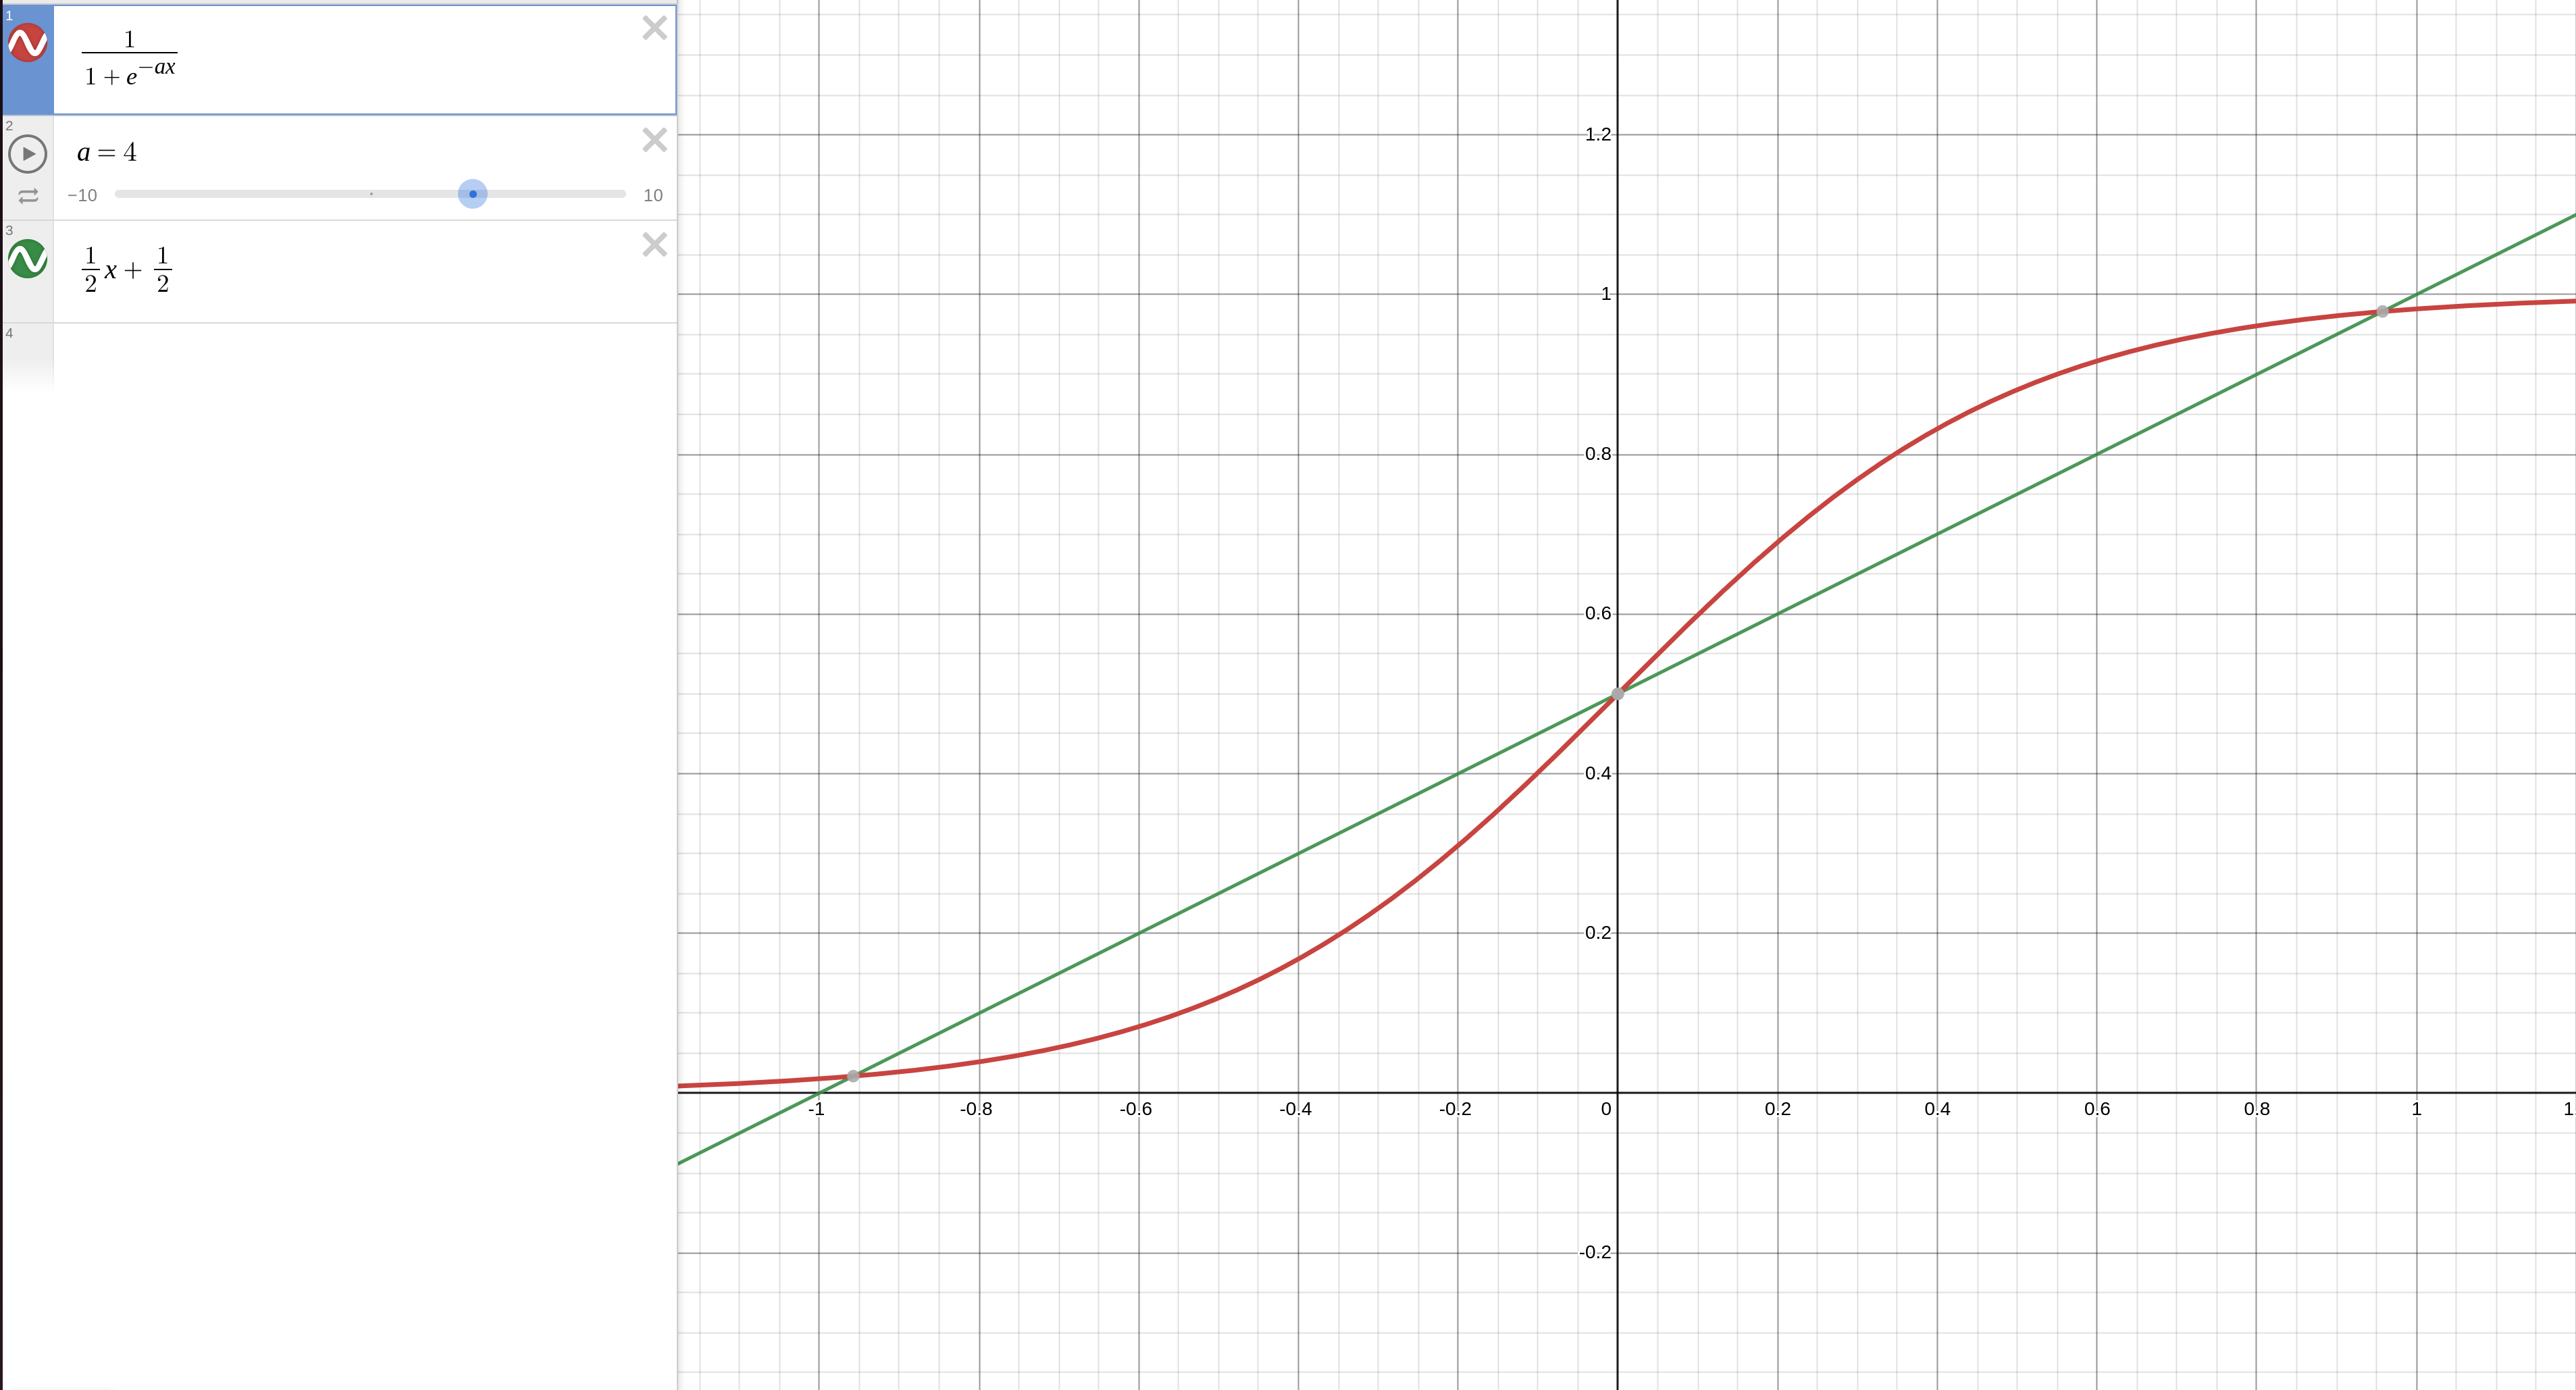
\includegraphics[width=0.7\linewidth]{sigmoid.png}
    \caption{$f(x)=\frac{1}{1+e^{-\alpha x}}$}
\end{figure}

\newpage
Therefore, we still test the performance of one pieces splines to fit these curve.
\subsection{Result}
\begin{figure}[h]
    \centering
    \subfigure[pieces = 1]{
        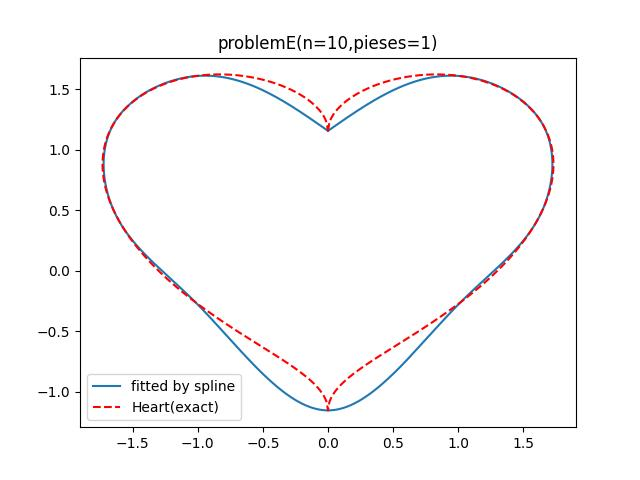
\includegraphics[width = 0.35\linewidth]{problemE(n=10,pieses=1).jpg}
    }
    \subfigure[pieces = 2]{
        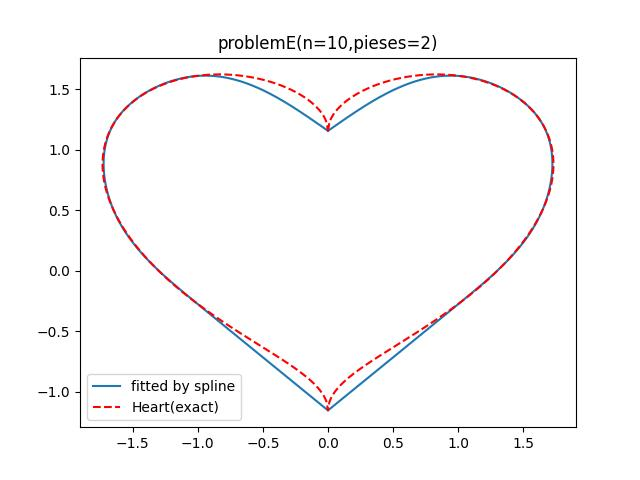
\includegraphics[width = 0.35\linewidth]{problemE(n=10,pieses=2).jpg}
    }
    \subfigure[pieces = 1,$\alpha=4$]{
        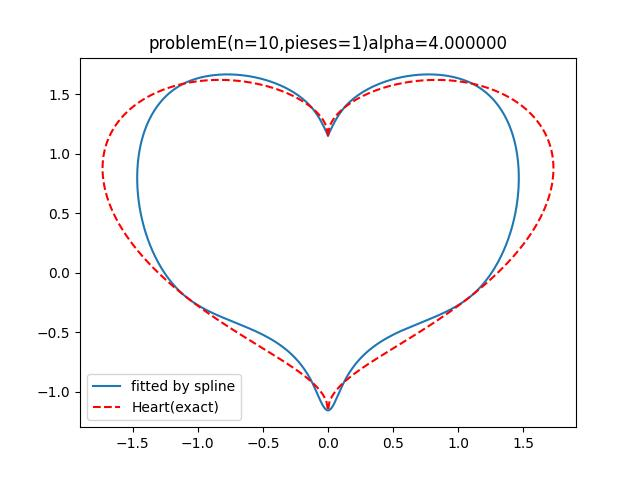
\includegraphics[width = 0.35\linewidth]{problemE(n=10,pieses=1)alpha=4.000000.jpg}
    }
    \subfigure[pieces = 2,$\alpha=4$]{
        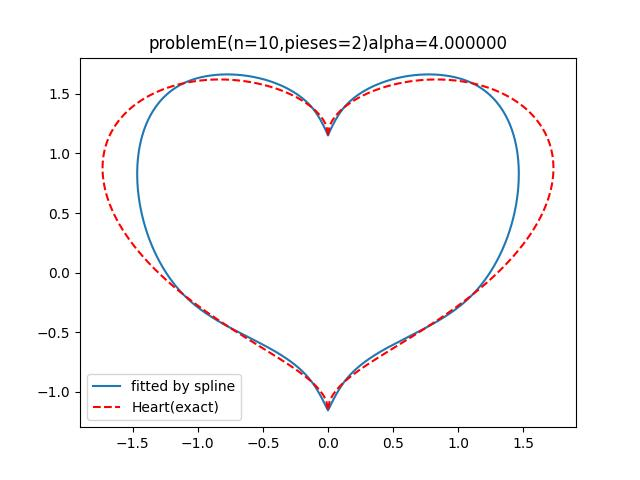
\includegraphics[width = 0.35\linewidth]{problemE(n=10,pieses=2)alpha=4.000000.jpg}
    }
    \caption{n=10}    
\end{figure}

Comparing the figure (a) and (b), we can find that 2 two pieces splines perform more excellent than one pieces near characteristic points, and performance of both of them are almost same at the other points.

Comparing the figure (a) (b) and (c) (d), we can find that the more knots near characteristic points much imporve the performance near the characteristic points, especially for one-pieces splines, though it will lose some information at the others points. Then let's see the result of $n = 40, 160$

\begin{figure}[h]
    \centering
    \subfigure[pieces = 1]{
        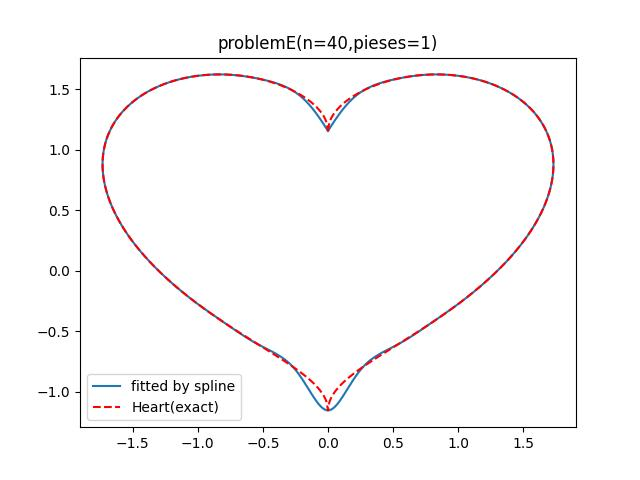
\includegraphics[width = 0.35\linewidth]{problemE(n=40,pieses=1).jpg}
    }
    \subfigure[pieces = 2]{
        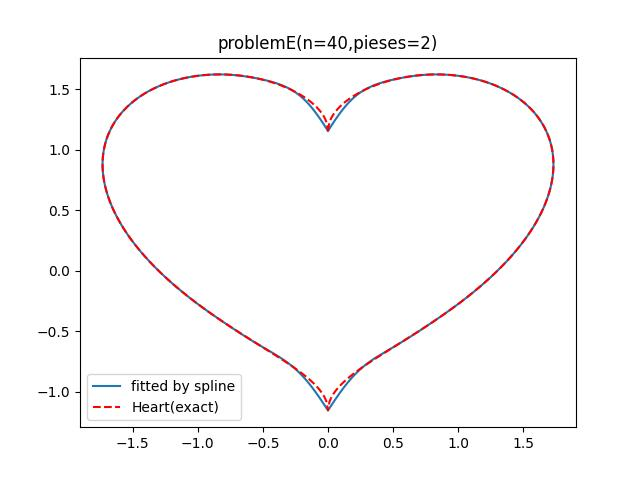
\includegraphics[width = 0.35\linewidth]{problemE(n=40,pieses=2).jpg}
    }
    \subfigure[pieces = 1,$\alpha=4$]{
        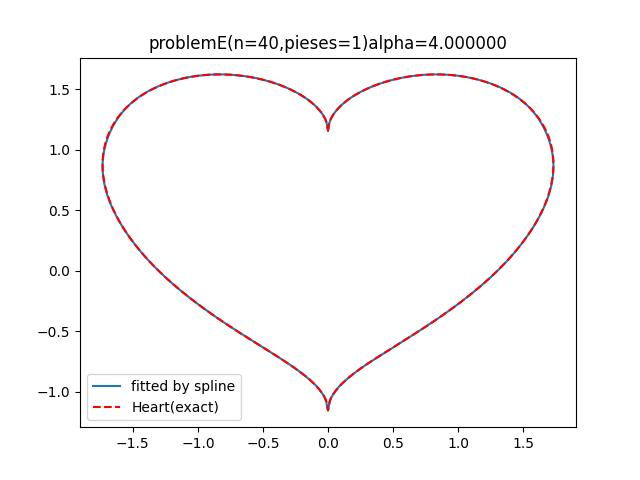
\includegraphics[width = 0.35\linewidth]{problemE(n=40,pieses=1)alpha=4.000000.jpg}
    }
    \subfigure[pieces = 2,$\alpha=4$]{
        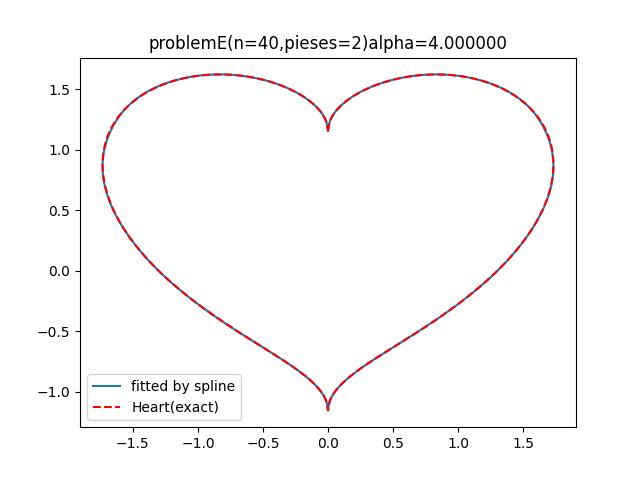
\includegraphics[width = 0.35\linewidth]{problemE(n=40,pieses=2)alpha=4.000000.jpg}
    }
    \caption{n=40}
    \subfigure[pieces = 1]{
        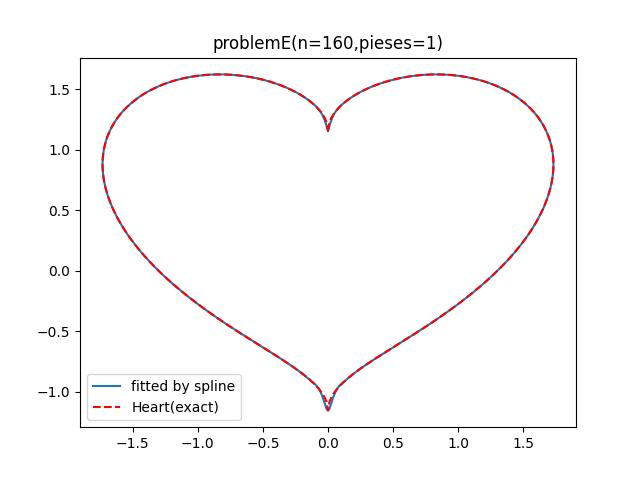
\includegraphics[width = 0.35\linewidth]{problemE(n=160,pieses=1).jpg}
    }
    \subfigure[pieces = 2]{
        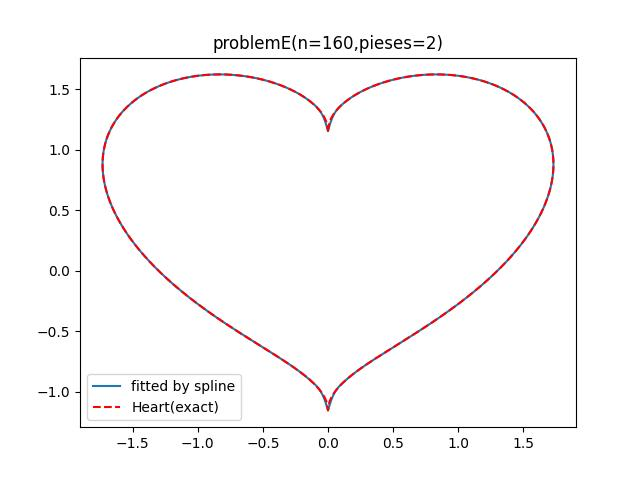
\includegraphics[width = 0.35\linewidth]{problemE(n=160,pieses=2).jpg}
    }
    \subfigure[pieces = 1,$\alpha=4$]{
        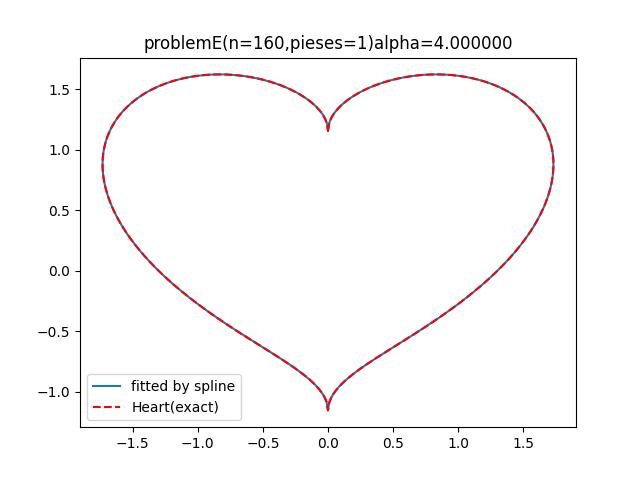
\includegraphics[width = 0.35\linewidth]{problemE(n=160,pieses=1)alpha=4.000000.jpg}
    }
    \subfigure[pieces = 2,$\alpha=4$]{
        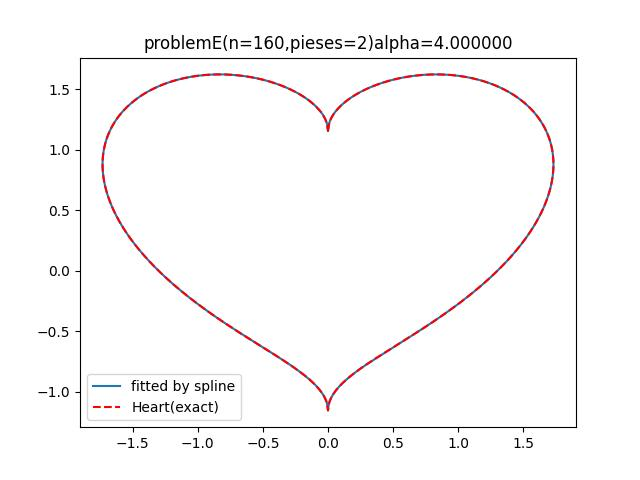
\includegraphics[width = 0.35\linewidth]{problemE(n=160,pieses=2)alpha=4.000000.jpg}
    }
    \caption{n=160}    
    From the figure above, the curve fitting can perform excellent enough with only 40 knots and one piece splines, if it choose more knots near the characteristic points, which is even better than 160 knots 
\end{figure}

% \newpage
% \section{Test for BSplines $\mathbb{S}_{n}^{n-1}$}

\end{document}
